\documentclass[12pt, a4paper]{article}

% Pakiety
\usepackage[utf8]{inputenc}
\usepackage[T1]{fontenc}
\usepackage[polish]{babel}
\usepackage{amsmath, amssymb}
\usepackage{graphicx}
\usepackage{float}
\usepackage{geometry}
\usepackage{hyperref}
\usepackage{booktabs}
\usepackage{caption}
\usepackage{listings}
\usepackage{xcolor}
\usepackage{parskip}

\geometry{
  a4paper,
  left=2.5cm,
  right=2.5cm,
  top=2.5cm,
  bottom=2.5cm
}

% Zakaz dzielenia wyrazów
\hyphenpenalty=10000
\exhyphenpenalty=10000
\emergencystretch=3em

\hypersetup{
  colorlinks=true,
  linkcolor=blue,
  urlcolor=blue,
  citecolor=blue
}

% Zmiana nazwy float figure: Rysunek -> Wykres
\addto\captionspolish{\renewcommand{\figurename}{Wykres}}

% Styl listingów
\lstset{
  language=Python,
  basicstyle=\ttfamily\small,
  keywordstyle=\color{blue}\bfseries,
  commentstyle=\color{gray}\itshape,
  stringstyle=\color{orange!80!black},
  numbers=left,
  numberstyle=\tiny\color{gray},
  numbersep=8pt,
  frame=single,
  breaklines=true,
  breakatwhitespace=true,
  captionpos=b,
  showstringspaces=false,
  columns=flexible,
  keepspaces=true,
  inputencoding=utf8,
  extendedchars=true,
  literate={ą}{{\k{a}}}1 {ę}{{\k{e}}}1 {ó}{{\'{o}}}1
            {ś}{{\'{s}}}1 {ł}{{\l{}}}1 {ź}{{\'{z}}}1
            {ż}{{\\.z}}1 {ć}{{\'{c}}}1 {ń}{{\'{n}}}1
            {Ą}{{\k{A}}}1 {Ę}{{\k{E}}}1 {Ó}{{\'{O}}}1
            {Ś}{{\'{S}}}1 {Ł}{{L}}1,
}

% Strona tytułowa
\title{
  \textbf{Metody Obliczeniowe w Nauce i Technice} \\[0.5em]
  \large Laboratorium 12: Równania różniczkowe cząstkowe
}
\author{Mateusz Stoch}
\date{10 czerwca 2026}

\begin{document}

\maketitle

% ============================================================
\section{Zadanie 1: Równanie eliptyczne -- Równanie Poissona}
% ============================================================

\textbf{Treść zadania:} Odkształcenia elastycznej membrany pod wpływem obciążenia o intensywności $f(x,y) = 8\pi^2 \sin(2\pi x)\cos(2\pi y)$ opisane są równaniem różniczkowym cząstkowym Poissona:
\[
  u_{xx} + u_{yy} = 8\pi^2 \sin(2\pi x)\cos(2\pi y)
\]
Dziedziną równania jest obszar $\Omega = [0,1]\times[0,1]$. Warunki brzegowe na brzegach dziedziny $\partial\Omega$ są następujące:
\[
  g(0,y) = g(1,y) = 0, \qquad g(x,0) = g(x,1) = \sin(2\pi x)
\]
Rozwiązaniem powyższego problemu jest funkcja $u(x,y) = \sin(2\pi x)\cos(2\pi y)$. Rozwiąż powyższe równanie stosując metodę różnic skończonych.

% ============================================================
\subsection{Zadanie 1(a): Dyskretyzacja operatorem pięciopunktowym}
% ============================================================

\textbf{Treść zadania:} Zastosuj operator pięciopunktowy do dyskretyzacji równań:
\[
  \nabla^2_5 = \frac{u_{i+1,j} - 2u_{i,j} + u_{i-1,j}}{h^2} + \frac{u_{i,j+1} - 2u_{i,j} + u_{i,j-1}}{k^2}
\]
gdzie $h = \Delta x$, $k = \Delta y$. Dla $h = k$ operator pięciopunktowy przyjmuje postać:
\[
  \nabla^2_5 = \frac{u_{i,j+1} + u_{i-1,j} - 4u_{i,j} + u_{i+1,j} + u_{i,j-1}}{h^2}
\]
gdzie $u_{i,j}$ oznacza rozwiązanie numeryczne w punkcie $(x_i, y_j)$. Przyjmij $h = 0{,}1$.

Zastosowano metodę różnic skończonych z krokiem $h = 0{,}1$. Dla siatki wewnętrznej o $N = 9$ węzłach w każdym kierunku powstaje układ $81 \times 81$. Do reprezentacji macierzy użyto formatu rzadkiego \texttt{lil\_matrix} z biblioteki \texttt{scipy.sparse}, a warunki brzegowe zostały wbudowane bezpośrednio w wektor prawej strony $b$.

\begin{lstlisting}[caption={Budowanie układu liniowego z operatora pięciopunktowego}]
def build_poisson_system(h):
    N = int(round(1/h)) - 1  # wezly wewnetrzne
    A = lil_matrix((N*N, N*N))
    b = np.zeros(N*N)
    for i in range(N):
        for j in range(N):
            k = i*N + j
            A[k, k] = -4.0
            b[k] = h**2 * f(xi, yj)
            if i+1 < N: A[k, (i+1)*N + j] = 1.0
            else:        b[k] -= g(1.0, yj)
            ...
    return csr_matrix(A), b, N
\end{lstlisting}

% ============================================================
\subsection{Zadanie 1(b): Wzorzec niezerowych elementów macierzy}
% ============================================================

\textbf{Treść zadania:} Zilustruj wzorzec z niezerowych elementów, jaki można zaobserwować w macierzy powstałej z zastosowania operatora pięciopunktowego. Przydatna będzie funkcja \texttt{spy}.

Wizualizacja struktury macierzy za pomocą funkcji \texttt{spy} (Wykres~\ref{fig:wykres1}) ujawnia na głównej przekątnej wartość $-4$, a bezpośrednie sąsiedztwo w obrębie każdego bloku i między blokami odpowiada wartościom $+1$.

\begin{figure}[H]
  \centering
  
\includegraphics[width=0.65\textwidth]{wykres1.png}
  \caption{Wzorzec niezerowych elementów macierzy Poissona ($h=0{,}1$, układ $81\times81$).}
  \label{fig:wykres1}
\end{figure}

% ============================================================
\subsection{Zadanie 1(c): Rozwiązanie iteracyjną metodą Conjugate Gradient}
% ============================================================

\textbf{Treść zadania:} Rozwiąż powstały układ równań liniowych, stosując wybraną przez siebie metodę iteracyjną.

Układ liniowy $Au = b$ rozwiązano metodą sprzężonych gradientów (\texttt{cg} z \texttt{scipy.sparse.linalg}). Ponieważ macierz $A$ jest ujemnie określona, do solvera przekazano $(-A)u = (-b)$, zapewniając symetrię i dodatniość macierzy.

Zbieżność osiągnięto po zaledwie 5 iteracjach, a końcowe residuum wyniosło $1{,}61 \cdot 10^{-14}$. Tak szybka zbieżność wynika z dobrze uwarunkowanej struktury macierzy dla tego zagadnienia. Przebieg normy residuum przedstawiono na Wykresie~\ref{fig:wykres2}.

\begin{figure}[H]
  \centering
  
\includegraphics[width=0.75\textwidth]{wykres2.png}
  \caption{Zbieżność metody Conjugate Gradient -- norma residuum w kolejnych iteracjach.}
  \label{fig:wykres2}
\end{figure}

% ============================================================
\subsection{Zadanie 1(d): Porównanie rozwiązania numerycznego z dokładnym}
% ============================================================

\textbf{Treść zadania:} Narysuj następujące wykresy: wykres funkcji $u(x,y)$, tj.\ dokładnego rozwiązania, oraz wykres funkcji $\hat{u}(x,y)$, tj.\ rozwiązania znalezionego metodą różnic skończonych; kolorowy wykres konturowy funkcji błędu.

Na Wykresie~\ref{fig:wykres3} zestawiono rozwiązanie dokładne $u(x,y) = \sin(2\pi x)\cos(2\pi y)$ z rozwiązaniem numerycznym $\hat{u}(x,y)$, a także kolorową mapę funkcji błędu $|u - \hat{u}|$.

Maksymalny błąd bezwzględny przy $h = 0{,}1$ wyniósł $3{,}50 \cdot 10^{-2}$, a średni $7{,}59 \cdot 10^{-3}$. Błąd jest wyraźnie większy w okolicach brzegu $y=0$ i $y=1$, gdzie funkcja ma największe gradienty.

\begin{figure}[H]
  \centering
  
\includegraphics[width=0.95\textwidth]{wykres3.png}
  \caption{Lewy panel: rozwiązanie dokładne (góra) i numeryczne (dół). Prawy panel: kolorowy wykres konturowy błędu $|u - \hat{u}|$.}
  \label{fig:wykres3}
\end{figure}

% ============================================================
\subsection{Zadanie 1(e): Empiryczny rząd zbieżności}
% ============================================================

\textbf{Treść zadania:} Wyznacz empiryczny rząd zbieżności operatora pięciopunktowego. W tym celu zastosuj we wzorze wartości $h$ od $1/4$ do $1/64$, zmniejszając $h$ o połowę w każdej iteracji.

Wyniki zestawiono w Tabeli~\ref{tab:zbieznosc}.

\begin{table}[H]
  \centering
  \caption{Maksymalny błąd bezwzględny oraz empiryczny rząd zbieżności dla różnych kroków $h$.}
  \label{tab:zbieznosc}
  \begin{tabular}{ccc}
    \toprule
    $h$ & Maks. błąd & Rząd $p$ (do poprzedniego) \\
    \midrule
    $1/4$  & $2{,}67 \cdot 10^{-1}$ & -- \\
    $1/8$  & $5{,}83 \cdot 10^{-2}$ & 2{,}19 \\
    $1/16$ & $1{,}41 \cdot 10^{-2}$ & 2{,}05 \\
    $1/32$ & $3{,}50 \cdot 10^{-3}$ & 2{,}01 \\
    $1/64$ & $8{,}73 \cdot 10^{-4}$ & 2{,}00 \\
    \bottomrule
  \end{tabular}
\end{table}

Średni empiryczny rząd zbieżności wynosi $p \approx 2{,}06$, co doskonale zgadza się z wartością teoretyczną $p = 2$ dla operatora pięciopunktowego. Oznacza to, że błąd dyskretyzacji spada proporcjonalnie do $h^2$ -- dwukrotne zagęszczenie siatki zmniejsza błąd czterokrotnie.

\begin{figure}[H]
  \centering
  
\includegraphics[width=0.75\textwidth]{wykres4.png}
  \caption{Maksymalny błąd bezwzględny w funkcji kroku $h$ w skali log-log. Nachylenie prostej potwierdza rząd 2.}
  \label{fig:wykres4}
\end{figure}

% ============================================================
\section{Zadanie 2: Równanie paraboliczne -- Równanie ciepła}
% ============================================================

\textbf{Treść zadania:} Dane jest równanie przewodnictwa ciepła:
\[
  u_t = u_{xx}, \qquad 0 \le x \le 1, \quad t \ge 0
\]
z warunkami początkowymi:
\[
  u(0, x) = \begin{cases} 2x & 0 \le x \le 0{,}5 \\ 2 - 2x & 0{,}5 \le x \le 1 \end{cases}
\]
oraz warunkami brzegowymi $u(t,0) = 0$, $u(t,1) = 0$.

% ============================================================
\subsection{Zadanie 2(a): Jawna metoda Eulera (FTCS)}
% ============================================================

\textbf{Treść zadania:} Zdyskretyzuj układ, zastępując $u_t$ różnicą progresywną oraz $u_{xx}$ różnicą centralną:
\[
  \frac{u_i^{k+1} - u_i^k}{\Delta t} = \frac{u_{i+1}^k - 2u_i^k + u_{i-1}^k}{(\Delta x)^2}
\]
Otrzymujemy stąd:
\[
  u_i^{k+1} = u_i^k + \frac{\Delta t}{(\Delta x)^2}\!\left(u_{i+1}^k - 2u_i^k + u_{i-1}^k\right)
\]
Przyjmij krok przestrzenny $\Delta x = 0{,}05$ oraz krok czasowy $\Delta t = 0{,}0012$, znajdź rozwiązanie dla czasu od $t=0$ do $t=0{,}06$. Narysuj wykres rozwiązania co dziesięć kroków czasowych. Stwórz wykres trójwymiarowy.

Dla podanych parametrów współczynnik stabilności wynosi $r = \Delta t / (\Delta x)^2 = 0{,}48 < 0{,}5$, co oznacza, że warunek stabilności von Neumanna jest spełniony i schemat jest stabilny. Na Wykresie~\ref{fig:wykres5} widać stopniowe wygładzanie się profilu temperatury -- ostry kształt namiotowy ulega rozlaniu i spłaszczeniu w czasie.

\begin{figure}[H]
  \centering
  
\includegraphics[width=0.95\textwidth]{wykres5.png}
  \caption{Ewolucja profilu temperatury metodą jawną FTCS ($\Delta t = 0{,}0012$, $r = 0{,}48$). Lewy panel: wykres powierzchniowy 3D, prawy: profile dla kolejnych kroków czasowych.}
  \label{fig:wykres5}
\end{figure}

% ============================================================
\subsection{Zadanie 2(b): Jawna metoda Eulera z krokiem $\Delta t = 0{,}0013$}
% ============================================================

\textbf{Treść zadania:} Powtórz obliczenia z poprzedniego punktu, przyjmując rozmiar kroku $\Delta t = 0{,}0013$. Stwórz nowy wykres, narysuj rozwiązanie analogicznie jak w podpunkcie (a). Wyjaśnij różnice w otrzymanym rozwiązaniu.

Dla $\Delta t = 0{,}0013$ współczynnik stabilności wynosi $r = 0{,}52 > 0{,}5$, co narusza warunek von Neumanna. Schemat jawny jest niestabilny -- błędy zaokrągleń narastają wykładniczo i rozwiązanie eksploduje, nie mając żadnego fizycznego sensu.

Wykres~\ref{fig:wykres6} wyraźnie ilustruje tę numeryczną eksplozję: zamiast wygładzonego profilu temperatury pojawia się oscylujące, gwałtownie rosnące rozwiązanie. Różnica między $\Delta t = 0{,}0012$ (stabilna) a $\Delta t = 0{,}0013$ (eksplozja) wynika z bardzo cienkiej granicy $r = 0{,}5$, której przekroczenie nawet o 4\% skutkuje zupełną utratą fizycznego sensu rozwiązania.

\begin{figure}[H]
  \centering
  
\includegraphics[width=0.95\textwidth]{wykres6.png}
  \caption{Numeryczna eksplozja rozwiązania przy $\Delta t = 0{,}0013$ ($r = 0{,}52 > 0{,}5$). Warunek stabilności von Neumanna nie jest spełniony.}
  \label{fig:wykres6}
\end{figure}

% ============================================================
\subsection{Zadanie 2(c): Niejawna metoda Eulera (BTCS)}
% ============================================================

\textbf{Treść zadania:} Rozwiąż ponownie równanie ciepła, tym razem używając metody niejawnej, opartej na niejawnej metodzie Eulera:
\[
  u_i^{k+1} = u_i^k + \frac{\Delta t}{(\Delta x)^2}\!\left(u_{i+1}^{k+1} - 2u_i^{k+1} + u_{i-1}^{k+1}\right)
\]
Przyjmij $\Delta x = 0{,}05$, ale użyj znacznie większego kroku czasowego $\Delta t = 0{,}005$. Znajdź rozwiązanie dla czasu od $t=0$ do $t=0{,}06$.

Powyższy schemat prowadzi do układu równań liniowych w każdym kroku czasowym:
\[
  (I - r \cdot D^2)\,\mathbf{u}^{k+1} = \mathbf{u}^k
\]
gdzie $D^2$ to macierz drugich różnic centralnych. Powstała macierz jest trójdiagonalna, symetryczna i dodatnio określona -- układ rozwiązano bezpośrednio (\texttt{spsolve}).

Kluczową zaletą metody niejawnej jest \textbf{bezwarunkowa stabilność}. W obliczeniach zastosowano znacznie większy krok czasowy $\Delta t = 0{,}005$, co daje współczynnik stabilności $r = 2{,}0$ (czterokrotne przekroczenie granicy stabilności metody jawnej). Jak widać na Wykresie~\ref{fig:wykres7}, rozwiązanie pozostaje w pełni stabilne i fizycznie poprawne, co potwierdza zalety schematów niejawnych.

\begin{figure}[H]
  \centering
  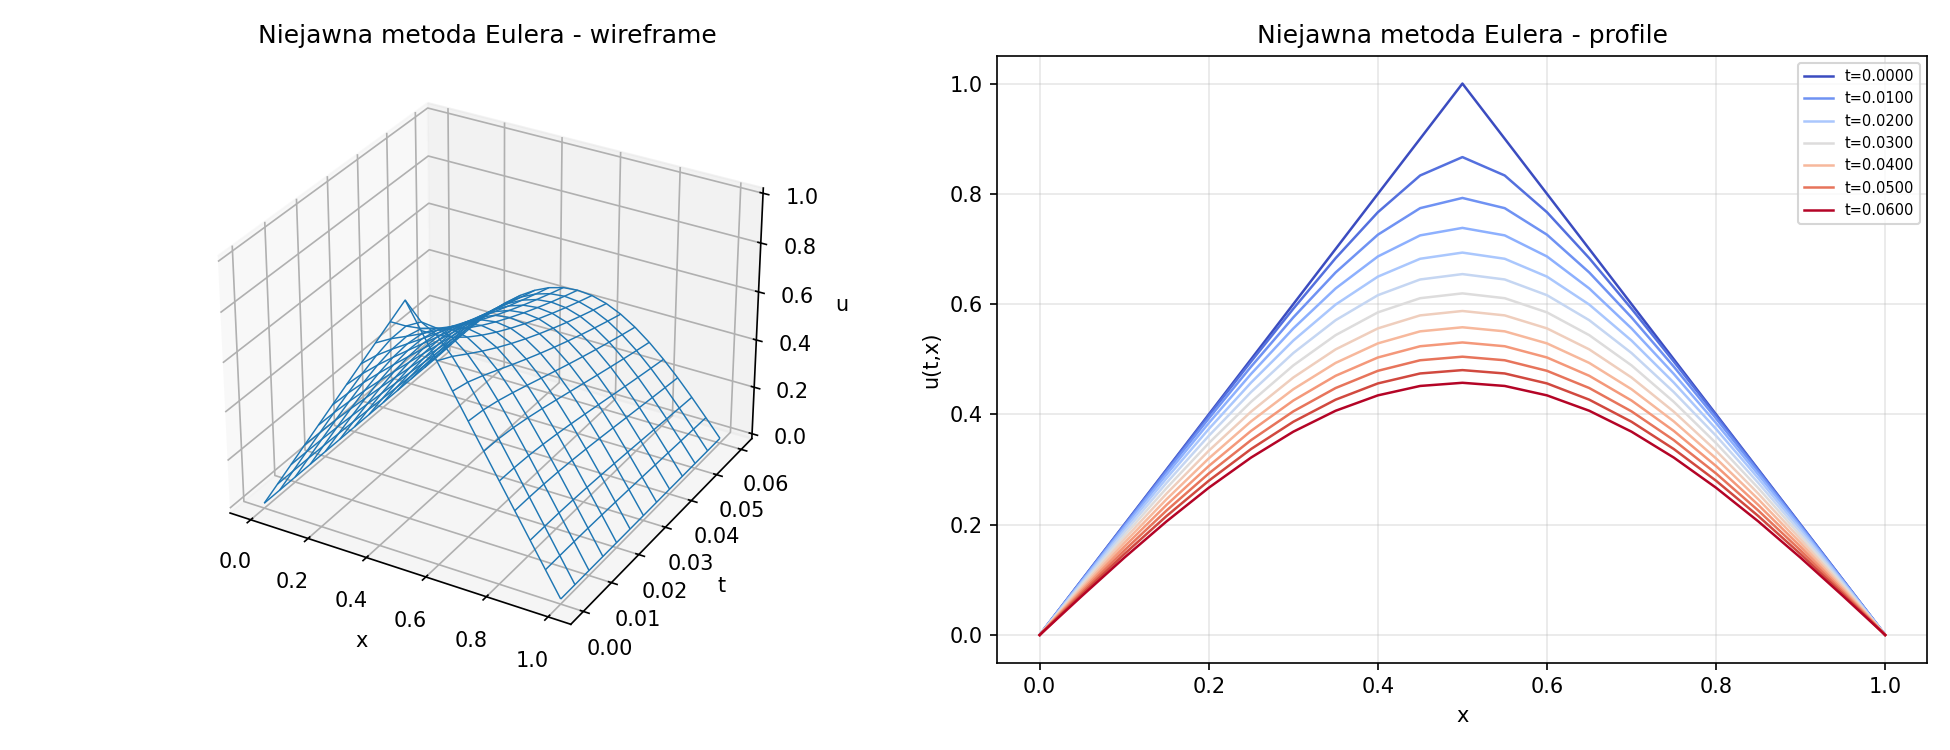
\includegraphics[width=0.95\textwidth]{wykres7.png}
  \caption{Stabilne rozwiązanie metodą niejawną BTCS przy dużym kroku czasowym ($\Delta t = 0{,}005$, $r = 2{,}0$).}
  \label{fig:wykres7}
\end{figure}

% ============================================================
\subsection{Zadanie 2(d): Metoda Cranka-Nicolson}
% ============================================================

\textbf{Treść zadania:} Rozwiąż jeszcze raz równanie, używając schematu Cranka-Nicolson, opartego na metodzie trapezów:
\[
  u_i^{k+1} = u_i^k + \frac{\Delta t}{2(\Delta x)^2} \left(u_{i+1}^{k+1} - 2u_i^{k+1} + u_{i-1}^{k+1} + u_{i+1}^k - 2u_i^k + u_{i-1}^k\right)
\]
Ponownie przyjmij $\Delta x = 0{,}05$ oraz $\Delta t = 0{,}005$ i znajdź rozwiązanie dla czasu od $t=0$ do $t=0{,}06$.

Schemat Cranka-Nicolson jest bezwarunkowo stabilną metodą o wyższym rzędzie dokładności -- $\mathcal{O}(\Delta t^2 + \Delta x^2)$ -- w porównaniu do niejawnej metody Eulera, która ma dokładność pierwszego rzędu w czasie. Prowadzi to do układu równań liniowych w każdym kroku czasowym:
\[
  \left(I - \frac{r}{2} D^2\right) \mathbf{u}^{k+1} = \left(I + \frac{r}{2} D^2\right) \mathbf{u}^k
\]
Macierz lewej strony (LHS) ma na głównej przekątnej wartości $1+r$, a na sąsiednich $-r/2$. Macierz prawej strony (RHS) ma na przekątnej $1-r$, a na sąsiednich $r/2$. Rozwiązanie wyznaczone dla $\Delta t = 0{,}005$ przedstawia Wykres~\ref{fig:wykres8}. Metoda ta doskonale wygładza profil i zachowuje stabilność.

\begin{figure}[H]
  \centering
  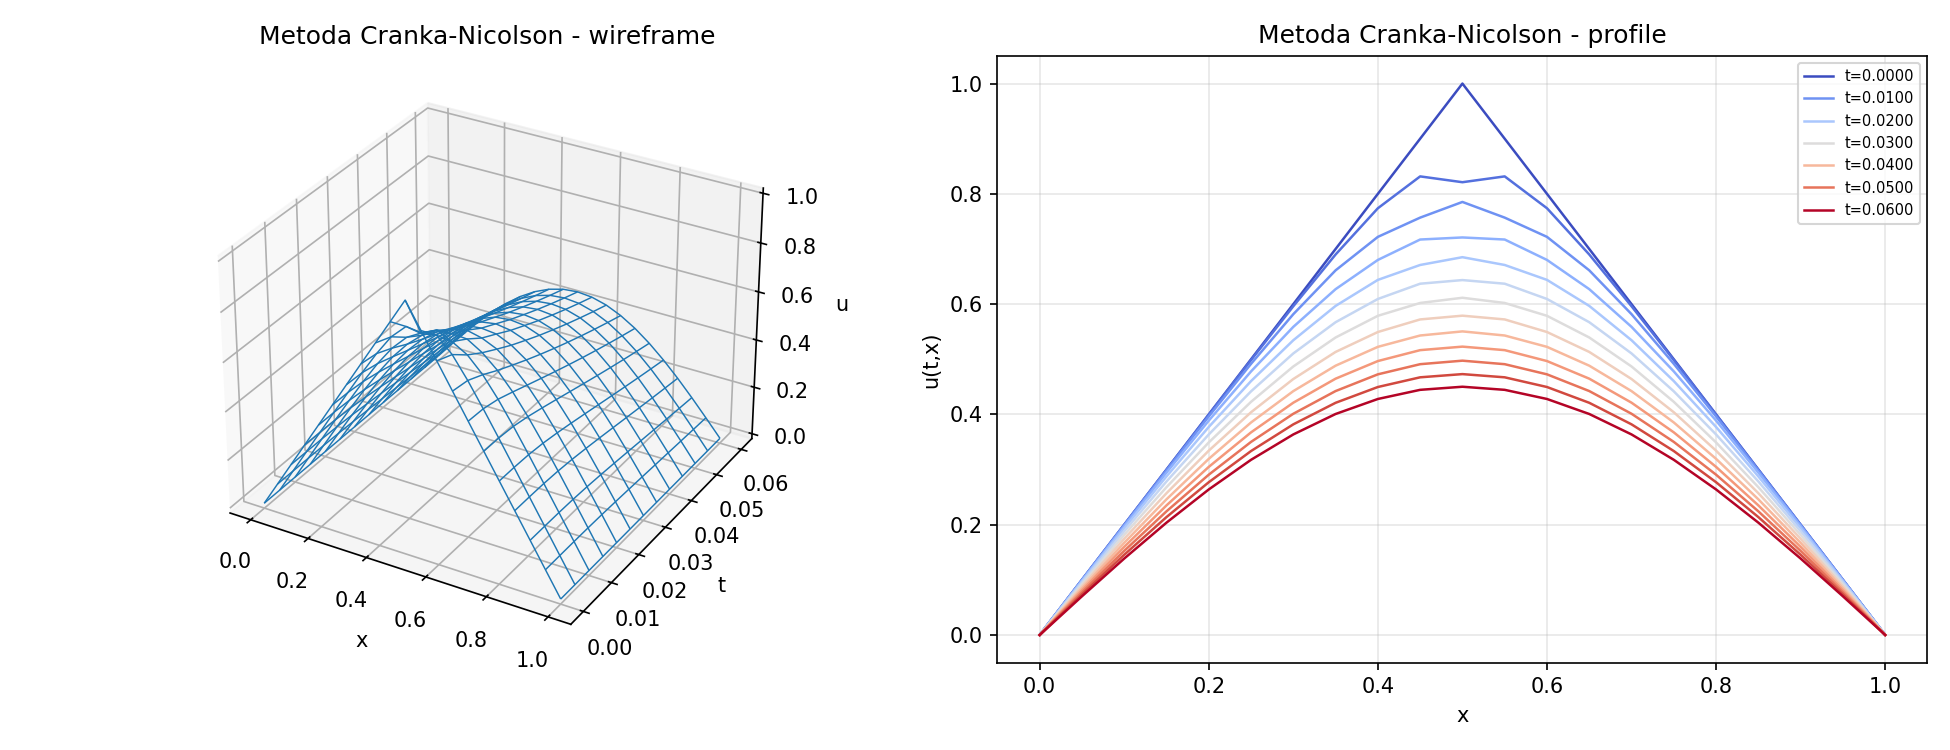
\includegraphics[width=0.95\textwidth]{wykres8.png}
  \caption{Rozwiązanie równania ciepła metodą Cranka-Nicolson ($\Delta t = 0{,}005$, $r = 2{,}0$).}
  \label{fig:wykres8}
\end{figure}

% ============================================================
\subsection{Zadanie 2(e): Metoda linii (MOL)}
% ============================================================

\textbf{Treść zadania:} Rozwiąż równanie metodą linii, dyskretyzując zmienną przestrzenną z krokiem $\Delta x = 0{,}05$, podczas gdy zmienna czasowa pozostaje ciągła. Uwzględniając sztywność układu, użyj odpowiedniego solwera na przedziale $0 \le t \le 0{,}06$.

Dyskretyzacja przestrzenna prowadzi do układu równań różniczkowych zwyczajnych (ODE):
\[
  \mathbf{y}'(t) = \frac{1}{(\Delta x)^2} M \mathbf{y}(t)
\]
gdzie $M$ jest macierzą trójdiagonalną ze współczynnikami $[-2, 1, 1]$. Ze względu na dużą rozpiętość wartości własnych macierzy (sztywność układu) zastosowano solver \texttt{Radau} (niejawna metoda Rungego-Kutty rzędu 5) z biblioteki \texttt{scipy.integrate.solve\_ivp}. Wyniki przedstawiono na Wykresie~\ref{fig:wykres9}.

\begin{figure}[H]
  \centering
  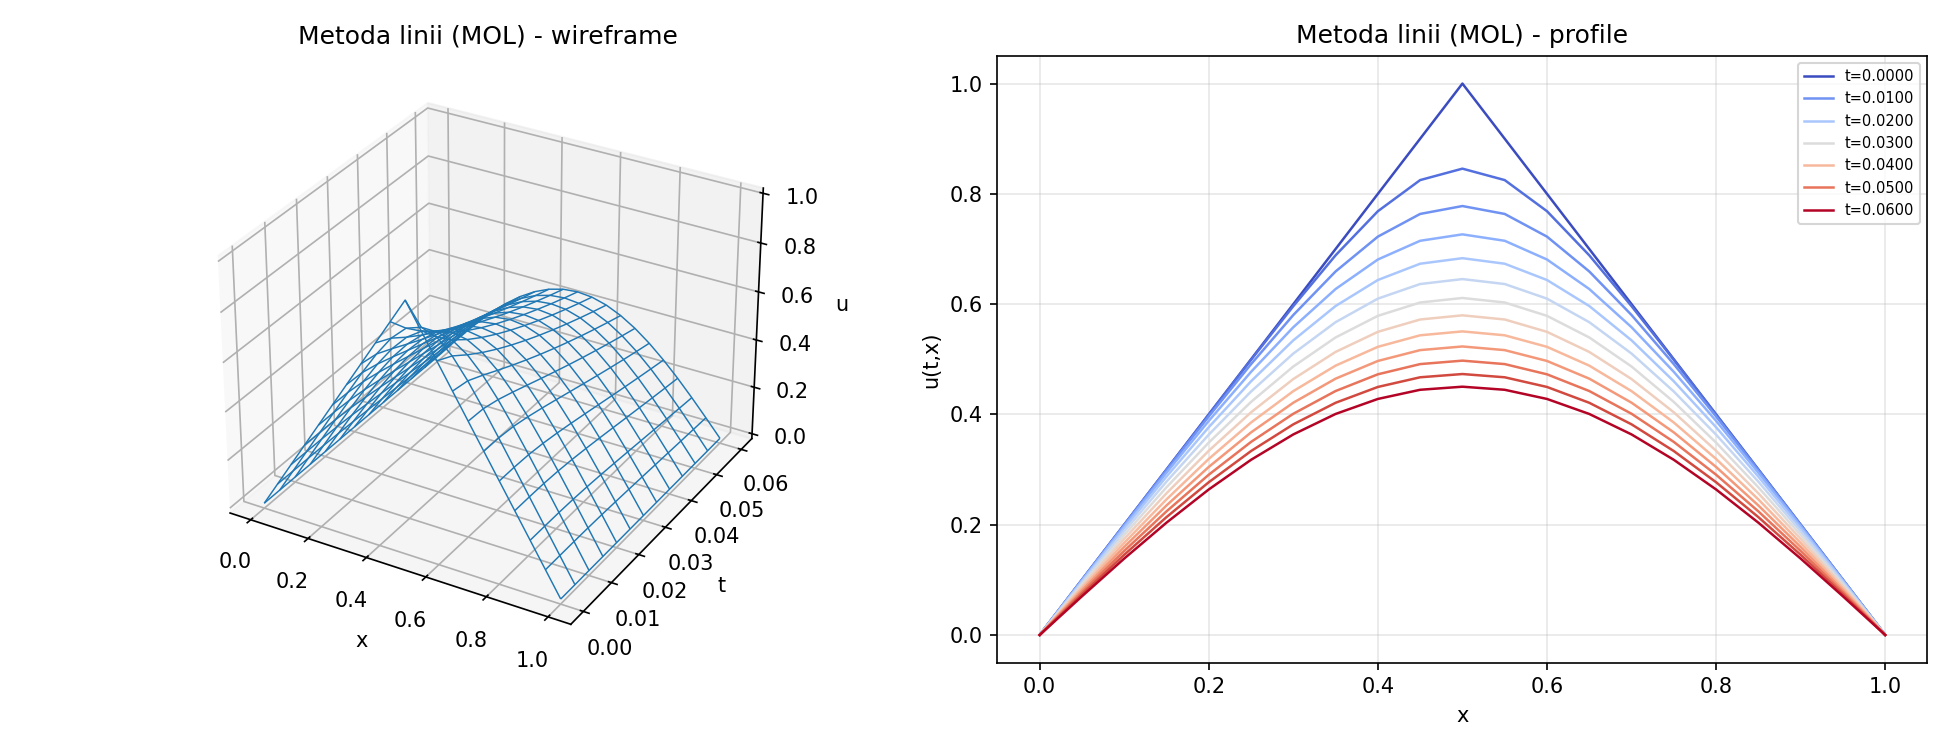
\includegraphics[width=0.95\textwidth]{wykres9.png}
  \caption{Rozwiązanie równania ciepła metodą linii (MOL) przy użyciu solvera Radau.}
  \label{fig:wykres9}
\end{figure}

% ============================================================
\subsection{Porównanie metod dla $t = 0{,}06$}
% ============================================================

Porównano wyniki uzyskane za pomocą metod: niejawnej Eulera (BTCS), Cranka-Nicolson (CN) oraz metody linii (MOL) dla końcowej chwili czasowej $t = 0{,}06$. Maksymalne różnice bezwzględne między rozwiązaniami wynoszą:
\begin{itemize}
  \item Niejawna Euler vs Crank-Nicolson: $7{,}16 \cdot 10^{-3}$
  \item Niejawna Euler vs Metoda linii: $7{,}09 \cdot 10^{-3}$
  \item Crank-Nicolson vs Metoda linii: $1{,}12 \cdot 10^{-4}$
\end{itemize}
Znikome różnice (szczególnie między Crank-Nicolson a metodą linii, które są schematami wyższego rzędu) potwierdzają poprawność wdrożenia wszystkich metod.

% ============================================================
\section{Wnioski}
% ============================================================

\begin{enumerate}
  \item Operator pięciopunktowy dla równania Poissona daje rząd zbieżności $p = 2$ względem kroku siatki $h$. Potwierdziły to obliczenia empiryczne (średnie $p \approx 2{,}06$). Metoda iteracyjna Conjugate Gradient była bardzo efektywna dla tej klasy układów, osiągając zbieżność w zaledwie 5 iteracjach.

  \item Jawna metoda Eulera (FTCS) dla równania ciepła wymaga spełnienia warunku von Neumanna $r = \Delta t / (\Delta x)^2 \le 0{,}5$. Jego naruszenie prowadzi do numerycznej eksplozji rozwiązania, co wyraźnie pokazało porównanie $\Delta t = 0{,}0012$ (stabilna) z $\Delta t = 0{,}0013$ (eksplozja).

  \item Metody niejawne (niejawna Eulera, Crank-Nicolson) oraz metoda linii (MOL) z niejawnycm solverem \texttt{Radau} są bezwarunkowo stabilne, co pozwala na stosowanie dużych kroków czasowych ($\Delta t = 0{,}005$, $r = 2{,}0$) bez obawy o stabilność rozwiązania.

  \item Metoda Cranka-Nicolson oraz metoda linii z wysokiego rzędu solverem dają dokładniejsze wyniki dzięki wyższemu rzędowi aproksymacji w czasie, co odzwierciedlają bardzo małe różnice między nimi ($\approx 1{,}12 \cdot 10^{-4}$).
\end{enumerate}

% ============================================================
\begin{thebibliography}{3}
  \bibitem{wikipedia_pde}
  Wikipedia, \emph{Partial differential equation}, \url{https://en.wikipedia.org/wiki/Partial_differential_equation} (dostęp: 10 czerwca 2026 r.).
  \bibitem{wikipedia_fdm}
  Wikipedia, \emph{Finite difference method}, \url{https://en.wikipedia.org/wiki/Finite_difference_method} (dostęp: 10 czerwca 2026 r.).
  \bibitem{leveque}
  R. J. LeVeque, \emph{Finite Difference Methods for Ordinary and Partial Differential Equations}, SIAM, 2007.
\end{thebibliography}

\end{document}
